\chapter{Testing}
%
Testen ist ein Prozess zum Nachweis der Qualitätsmerkmale eines
Produktes.
\begin{itemize}
\item Testen wird mit der Absicht ausgeführt,
jeden erdenklichen Fehler oder Schwachstelle in einem Produkt zu finden.
\item Kein Programm kann so getestet werden, dass seine Fehlerfreiheit
garantiert ist.
\item Testen ist ebenso destruktiv wie
  kreativ und intellektuell herausfordernd.
\item Testen heisst: Verifizieren + Validieren.
\item Mit Tests können nur Symptome gefunden werden nicht jedoch Ursachen.
\end{itemize}
\ifslides
\newpage
\fi
Grunds\"atze:
\begin{itemize}
\item Alle Phasen der Entwicklung umfassen.
\item Selber geschriebene Programme nicht selber testen.
\item Resultate vorher festlegen.
\item Ergebnisse seri\"os \"uberpr\"ufen.
\item Testdaten auch f\"ur ung\"ultige und unerwartete Eingaben auslegen.
\item Tests mit Zufallsdaten vermeiden. % (keine Reproduzierbarkeit).
\item Keine Wegwerftests entwerfen.
\end{itemize}
\newslide
\begin{figure}[H]
\begin{center}
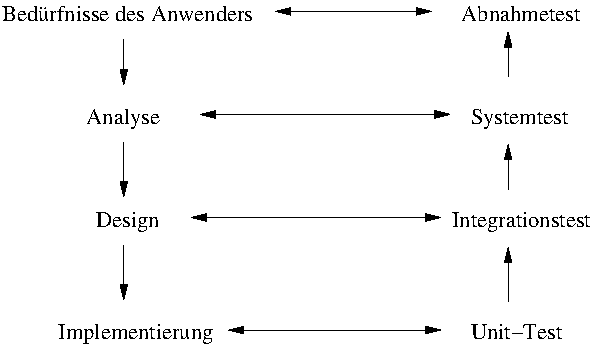
\includegraphics[width=0.8\linewidth]{qm/xfig/testlevels}
\caption{Die Test- und Entwicklungsphasen}
\end{center}
\end{figure}
\newslide
\section{Status Quo des Testens}
Testen ist typischerweise (Zitat Frank Westphal)
\begin{itemize}
\item  die letzte Phase in wasserfallartigen Projekten,
\item das letzte Kapitel in Büchern über Software-Engineering,
\item etwas, worauf kaum ein Programmierer wirklich Lust hat,
\item Aufgabe der Abteilung für Qualitätssicherung,
\item schmerzhaft, wenn wir Fehler lange nach ihrer Entstehung finden,
\item das Erste, was über Bord geht, wenn es eng wird,
\item nur ad hoc, selten systematisch.
\end{itemize}
\newslide
Effektives Testen muss:
\begin{itemize}
\item zeitnah zur Programmierung erfolgen,
\item automatisiert wiederholbar,
\item Spass machen,
\item so häufig wie Kompilieren ausgeführt werden,
\item so einfach wie Kompilieren sein,
\item pragmatisch sein,
\item mehr bringen als kosten.
\end{itemize}
\newslide
%%
\section{Begriffe (IEEE 610.12-90)}
\begin{description}
\item[Failure] (Fehlerwirkung, Ausfall, Störung)
   Abweichung vom spezifizierten oder nachweisbar korrekten Betriebsverhalten.
 \item[Fault] (Bug, Fehlerzustand, Defekt)
   Ursache einer oder mehrerer Störungen.
 \item[Error] (Fehler)
   Diskrepanz zwischen einem berechneten und dem korrektem Wert
 \item[Mistake] (Fehlhandlung)
   falsche, unkorrekte oder unvollständige Implementierung
\end{description}
\ifslides
\newpage
\fi
% Begriffe:
% - error (Fehler)
%       discrepancy between a computed, observed or measured value
%       and the true, specified, or theoretically correct value
% - fault (Defekt)
%       a condition that causes the software to fail to perform
%       its required function (bug)
% - failure (Versagen)
%       inability of a system to perform a required function
%       according to its specification.
%
%\newpage
\section{Vorgehen}
%
\ifslides
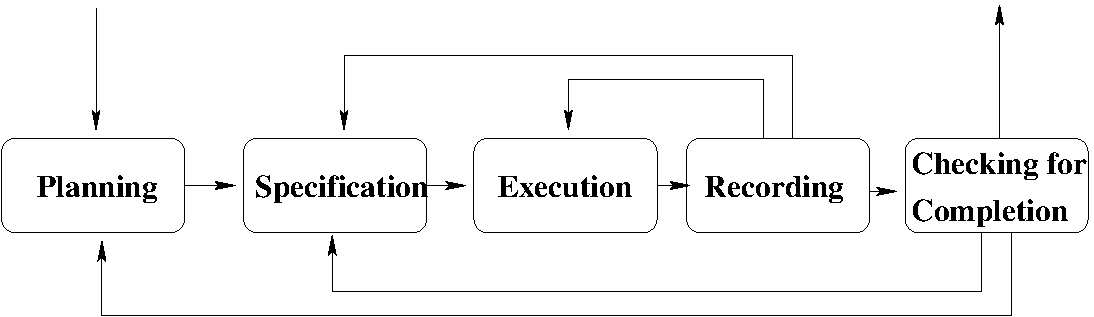
\includegraphics[width=\linewidth]{qm/xfig/testprocess}\\
\newslide
\else
\begin{figure}[H]
\begin{center}
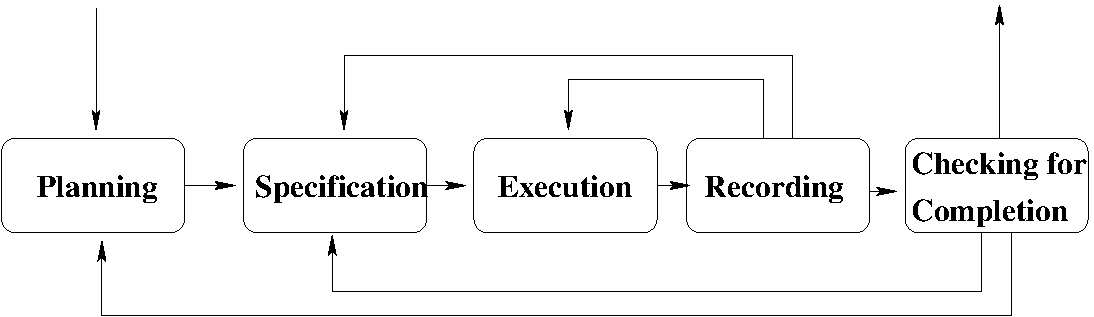
\includegraphics[width=0.7\linewidth]{qm/xfig/testprocess}\\
\end{center}
\caption{Der Testprozess nach BS 7925-2}
\end{figure}
\fi
%
\begin{enumerate}
\item \underline{Testplanung:}
Ressourcen und Zeit setzen dem Testaufwand Grenzen. Effektives Testen
muss geplant werden und alle Schichten des Systems abdecken:
\begin{itemize}
\item Festlegung einer Teststrategie: optimale Verteilung des Testaufwands auf
  die zentralen, kritischen Teile des Softwaresystemes,
  d.h. diejenigen mit der grössten Auswirkung. Priorisierung der Tests
\item Festlegung der Testabschluss-Kriterien: Überdeckungsgrad (code
  coverage): Der Anteil der zu
  testenden Funktionen, Klassen, GUI-Elemente, Verzweigungen, Kodezeilen.
\item Festlegung des Zeitplanes und der Zuständigkeiten.
\item Implementierung und Konfiguration der Testumgebung.
\end{itemize}
\ifslides
\newpage
\fi
\item \underline{Testspezifikation:} Festlegung der Testfälle, Testkriterien (pass/fail
  criteria), Testverfahren und -werkzeuge
  \begin{itemize}
  \item Prüfung der Soll-Ergebnisse
  \item Prüfung des Verhaltens bei unerwarteten, ungültigen Eingaben
  bzw. Randbedingungen (exception handling)
  \end{itemize}
\item \underline{Testdurchführung:}
  Installation des Testobjektes, Prüfung auf Vollständigkeit, Durchführung
  gem. festgelegter Teststrategie, Testabbruch bei schwerwiegenden Mängeln
\ifslides
\newpage
\fi
\item \underline{Testprotokollierung (Aufzeichnung):} Wer hat was, wann, wie und mit
  welchem Ergebnis getestet, Sicherstellung der Nachvollziehbarkeit, Nachweis
  der Durchführung.
\item \underline{Testauswertung:} Analyse der Testergebnisse, Priorisierung der
  Fehlerbehebung, Entscheid über Testabschluss, Evaluation des Testprozesses.
\end{enumerate}
%
\newpage
\section{Testmethoden}
%\begin{longtable}{|p{4.5cm}|p{4.5cm}|p{5cm}|p{1cm}|} \hline
\begin{tabularx}{\linewidth}{l|X}
%\hline
 Black-Box-Test &datengetriebenes Ein-Ausgabe-Testen. Die Testdaten
werden anhand der Spezifikation erzeugt.\\
 White-Box-Test & logisch-orientiertes Testen.
Alle Programmpfade m\"ussen mindestens einmal durchlaufen werden.\\
 Kode-Inspektionen & Gemeinsame Fehlersuche im Programmkode anhand formaler Kriterien.\\
 Walkthroughs & Das Testteam ist der Computer: informale, mehr oder weniger
 spontane Durchführung verschiedener Ablaufszenarien.\\
 Peer ratings & Gegenseitige Beurteilung der Programme in der Gruppe.\\
 Unit-Test & Testen einzelner Funktionen oder Code-Modulen (Klassen).\\
Integrations-Test & Testen (inkrementell) zusammengefügter Teile
    einer Applikation.\\
%\ifslides
%\end{tabularx}
%\newpage
%\begin{tabularx}{\linewidth}{l|X}
%\fi
 Funktions-Test & Testen funktionaler Anforderungen einer
  Applikation.\\
 System-Test & Testen des vollständig realisierten Systems unter
  möglichst realen Bedingungen.\\
 Regressions-Test & wiederholtes Testen nach vorgenommenen Korrekturen
  oder \"Anderungen.\\
 Abnahme-Test & beim Auftraggeber durchgeführtes Testen vor
   der produktiven Einführung des Systems.\\
 Last-Test & (auch Stress- od. Performanz-Test) Testen des
  Systemverhaltens unter ausserordentlichen Belastungsbedingungen.\\
 Usability-Test & Testen der Bedienerfreundlichkeit.\\
 Installations-Test & Testen des Installationsprozesses.\\
 Recovery-Test & Test der Wiederherstellbarkeit nach erfolgtem
  Systemunterbruch.\\
\newslide
%\ifslides
%\end{tabularx}
%\newpage
%\begin{tabularx}{\linewidth}{l|X}
%\fi
 Sicherheits-Test & Testen der Schutzmechanismen gegen Datenverlust
    oder unerlaubte Lese- und Schreibzugriffe.\\
 Kompatibilitäts-Test & Testen in bestimmten Software-/Hardware-Umgebungen\\
 exploratives Testen & nicht geplantes, informelles Testen mit dem
  Zweck, das System kennenzulernen.\\
\end{tabularx}
\newpage
\begin{tabularx}{\linewidth}{l|X}
 Vergleichs-Test & Vergleich der Stärken und Schwächen eines Systems
    mit Konkurrenzprodukten.\\
  Alpha-/Beta-Test & Von Anwendern durchgeführte Tests kurz vor
  Entwicklungsabschluss, wenn nur noch wenig Korrekturen und Anpassungen
  erwartet werden.\\
 Mutations-Test &\"Uberprüfung der Testfälle
  durch gezielten Einbau von Fehlern. (Fehler-Injektions-Test) \\
\end{tabularx}
%
%\newpage
\section{Dokumentation}
%       \addcontentsline{toc}{subsection}{Dokumentation}
% wikipedia!
\begin{figure}[H]
\centering
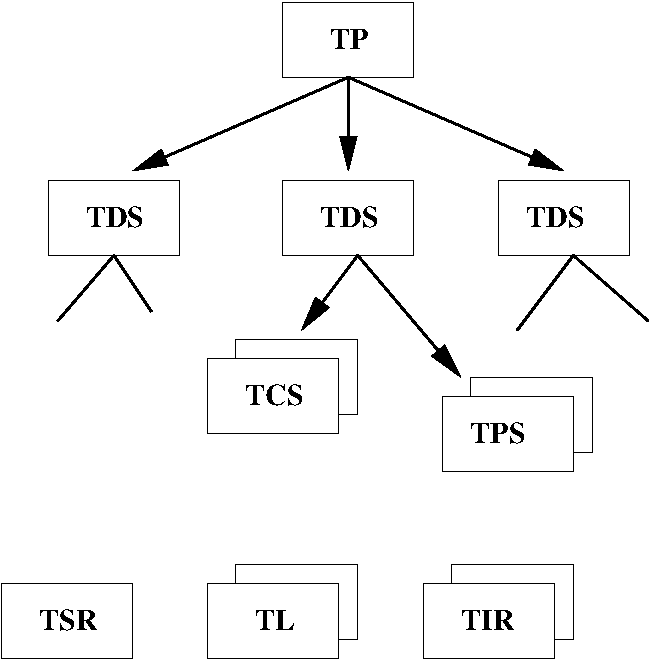
\includegraphics[width=0.6\linewidth]{qm/xfig/ieee829}
\ifslides
\else
\caption{Struktur der Testdokumente nach IEEE 829-1998}
\fi
\end{figure}
\begin{description}
\item[TP] Test Plan (Testplan): Beschreibung der Vorgehensweise, des Umfanges
  (zu testende Funktionalität), der Ressourcen, des Zeitplanes, der
  Verantwortlichkeiten.
\item[TDS] Test Design Specification (Testentwurfsspezifikation):
  Konkretisierung des Vorgehens, Testtechniken, Werkzeuge,
  Entscheidungskriterien (pass/fail criteria).
\item[TCS] Test Case Specification: eine Kombination von Eingaben und
  erwarteten Ausgaben.
\item[TPS] Test Procedure Specification (Testverfahrensspezifikation):
  schrittweise Anleitung zur Testdurchführung, Art der Messungen,
  Aufzeichnungsformat der Ergebnisse.
\ifslides
\newpage
\fi
\item[TL] Test Log (Testprotokoll): chronologische Auflistung der Ereignisse
  (Beginn und Ende der Testdurchführung, Ergebnisse, Ausgaben, Abweichungen),
  beteiligte Personen.
\item[TIR] Test Incident Report (Testvorfallbericht): Dokumentation
  spezieller, näher zu analysierenden Vorkommnisse während der
  Testdurchführung.
\item[TS] Test Summary (Testergebnisbericht): Entscheid, ob bestanden oder
  nicht (passed/failed).
\end{description}
\newpage
%-------------------------------------------------------------------------
%\kopf
%\section*{Methodisches Testen}
\section{Kode-Inspektionen}
%       \addcontentsline{toc}{subsection}{Kode-Inspektionen}
Das Lesen und die visuelle \"Uberpr\"ufung des Programms durch ein Testteam.
\vspace{1cm}

\begin{tabular}{p{4.5cm}p{10.5cm}}
Teilnehmer & T\"atigkeiten \\ \hline
\raisebox{-4ex}{\textbf Moderator} & \begin{itemize}
                                \item Verteilung der Unterlagen,
                                \item Zeitplanung,
                                \item Sitzungsleitung,
                                \item Kontrolle der Fehlerkorrekturen
                                \end{itemize}\\
\raisebox{-4ex}{\textbf Programmautor(en)} & \begin{itemize}
                                        \item Vorstellung und Erkl\"arung des
                                                 Programmes
                                        \end{itemize}\\
\raisebox{-4ex}{\textbf 2-3 Fachspezialisten} & \begin{itemize}
                                        \item Fehlersuche (keine Korrekturen!)
                                        \end{itemize}\\
\end{tabular}

\begin{itemize}
\item Dauer: jeweils 90 - 120 Minuten (ca. 150 Zeilen)
\item Hilfsmittel: Checklisten% (z.B. Christopher Fox)
\item Siehe auch \href{http://www.reviewtechnik.de/checklisten.html}
  {www.reviewtechnik.de/checklisten.html}
\end{itemize}
\newpage
%-------------------------------------------------------------------------
%\kopf
%\section*{Methodisches Testen}
\subsection{Java Inspection Checklist}
%       \addcontentsline{toc}{subsection}{Fehler-Checkliste}
%Die Erfahrung zeigt, dass immer wieder die gleichen Fehler gemacht werden.
\begin{enumerate}
\item {\textbf Variable, Attribute, and Constant Declaration Defects (VC):}
\begin{enumerate}
\item Are descriptive variable and constant names used in accord with naming
  conventions?
\item Are there variables or attributes with confusingly similar names?
%\item Is every variable and attribute correctly typed?
\item Is every variable and attribute properly initialized?
%\item Could any non-local variables be made local?
\item Are all for-loop control variables declared in the loop header?
\item Are there literal constants that should be named constants?
\item Are there variables or attributes that should be constants?
\item Are there attributes that should be local variables?
\item Do all attributes have appropriate access modifiers (private, protected,
  public)?
\item Are there static attributes that should be non-static or vice-versa?
\end{enumerate}
\ifslides
\newpage
\fi
\item {\textbf Method Definition Defects (FD):}
  \begin{enumerate}
  \item Are descriptive method names used in accord with naming conventions?
  \item Is every method parameter value checked before being used?
  \item For every method: Does it return the correct value at every method
  return point?
  \item Do all methods have appropriate access modifiers (private, protected,
  public)?
  \item Are there static methods that should be non-static or vice-versa?
  \end{enumerate}
\item {\textbf Class Definition Defects (CD):}
  \begin{enumerate}
  \item Does each class have appropriate constructors? % and destructors?
  \item Do any subclasses have common members that should be in the
  superclass?
\item Can the class inheritance hierarchy be simplified?
  \end{enumerate}
\ifslides
\newpage
\fi
\item {\textbf Data Reference Defects (DR):}
  \begin{enumerate}
  \item For every array reference: Is each subscript value within the defined
  bounds?
\item For every object or array reference: Is the value certain to be
  non-null?
  \end{enumerate}
\item {\textbf Computation/Numeric Defects (CN):}
  \begin{enumerate}
  \item Are there any computations with mixed data types?
  \item Is overflow or underflow possible during a computation?
  \item For each expressions with more than one operator: Are the assumptions
  about order of evaluation and precedence correct?
\item Are parentheses used to avoid ambiguity?
  \end{enumerate}
\ifslides
\newpage
\fi
\item {\textbf Comparison/Relational Defects (CR):}
  \begin{enumerate}
  \item For every boolean test: Is the correct condition checked?
  \item Are the comparison operators correct?
  \item Has each boolean expression been simplified by driving negations
  inward?
\item Is each boolean expression correct?
\item Are there improper and unnoticed side-effects of a comparison?
\item Has an \verb+&+ inadvertently been interchanged with a \verb+&&+ or a
  \verb+|+ for a \verb+||+?
  \end{enumerate}
\ifslides
\newpage
\fi
\item {\textbf Control Flow Defects (CF):}
\begin{enumerate}
\item For each loop: Is the best choice of looping constructs used?
\item Will all loops terminate?
\item When there are multiple exits from a loop, is each exit necessary and
  handled properly?
\item Does each switch statement have a default case?
\item Are missing switch case break statements correct and marked with a
  comment?
\item Do named break statements send control to the right place?
\item Is the nesting of loops and branches too deep, and is it correct?
\item Can any nested if statements be converted into a switch statement?
\item Are null bodied control structures correct and marked with braces or
  comments?
\item Are all exceptions handled appropriately?
\item Does every method terminate?
\end{enumerate}
\ifslides
\newpage
\fi
\item {\textbf Input-Output Defects (IO):}
  \begin{enumerate}
  \item Have all files been opened before use?
  \item Are the attributes of the input object consistent with the use of the
  file?
\item Have all files been closed after use?
\item Are there spelling or grammatical errors in any text printed or
  displayed?
\item Are all I/O exceptions handled in a reasonable way?
  \end{enumerate}
\item {\textbf Module Interface Defects (MI):}
\begin{enumerate}
\item Are the number, order, types, and values of parameters in every method
  call in agreement with the called method's declaration?
\item Do the values in units agree (e.g., inches versus yards)?
\item If an object or array is passed, does it get changed, and changed
  correctly by the called method?
\end{enumerate}
\ifslides
\newpage
\fi
\item {\textbf Comment Defects (CM):}
  \begin{enumerate}
  \item Does every method, class, and file have an appropriate header comment?
  \item Does every attribute, variable, and constant declaration have a
  comment?
\item Is the underlying behavior of each method and class expressed in plain
  language?
\item Is the header comment for each method and class consistent with the
  behavior of the method or class?
\item Do the comments and code agree?
\item Do the comments help in understanding the code?
\item Are there enough comments in the code?
\item Are there too many comments in the code?
  \end{enumerate}
\ifslides
\newpage
\fi
\item {\textbf Layout and Packaging Defects (LP):}
  \begin{enumerate}
  \item Is a standard indentation and layout format used consistently?
  \item For each method: Is it no more than about 60 lines long?
  \item For each compile module: Is no more than about 600 lines long?
  \end{enumerate}
\item {\textbf Modularity Defects (MO):}
  \begin{enumerate}
  \item Is there a low level of coupling between modules (methods and
  classes)?
\item Is there a high level of cohesion within each module (methods or class)?
\item Is there repetitive code that could be replaced by a call to a method
  that provides the behavior of the repetitive code?
\item Are the Java class libraries used where and when appropriate?
  \end{enumerate}
\ifslides
\newpage
\fi
\item {\textbf Storage Usage Defects (SU):}
  \begin{enumerate}
  \item Are arrays large enough?
  \item Are object and array references set to null once the object or array
  is no longer needed?
  \end{enumerate}
\item {\textbf Performance Defects (PE)} {(\em Optional)}:
  \begin{enumerate}
  \item Can better data structures or more efficient algorithms be used?
  \item Are logical tests arranged such that the often successful and
  inexpensive tests precede the more expensive and less frequently successful
  tests?
\item Can the cost of recomputing a value be reduced by computing it once and
  storing the results?
\item Is every result that is computed and stored actually used?
\item Can a computation be moved outside a loop?
\item Are there tests within a loop that do not need to be done?
\item Can a short loop be unrolled?
\item Are there two loops operating on the same data that can be combined into
  one?
%\item Are frequently used variables declared register?
%\item Are short and commonly called methods declared inline?
  \end{enumerate}
\end{enumerate}
{\em Quelle: Christopher Fox, James Madison University, Harrisonburg, VA}

(leicht angepasst an Java)
\newpage
\section{Testfall-Spezifikation}
Beispiel:
\begin{lstlisting}[language=java]
  double M( double A, double B, double X ){
    if( (A > 1) && (B == 0) ) {
      X = X/A;
    }
    if( (A == 2) || (X > 1) ) {
      X= X+1;
    }
    return X;
  }
\end{lstlisting}
\ifslides
\begin{center}
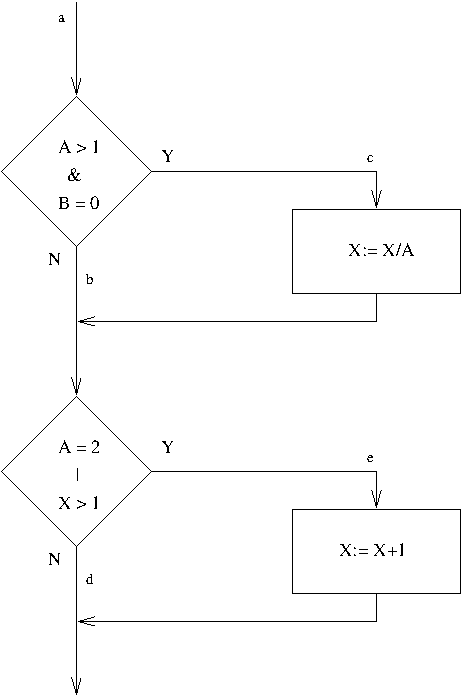
\includegraphics[width=0.4\linewidth]{qm/xfig/testfall}
\end{center}
\else
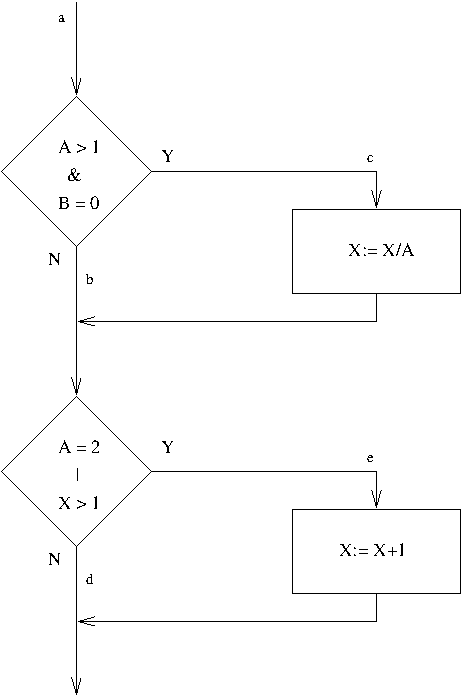
\includegraphics{qm/xfig/testfall}
\fi
\newpage
%-------------------------------------------------------------------------
%\subsection{Testfall-Spezifikation}
\begin{center}
\begin{tabular}{|p{5cm}|p{5cm}|}
\hline
\multicolumn{2}{|c|}{\bfseries\large Testfall-Spezifikation}\\
\hline
       Programm:   &  Modul/Prozedur : \\
    Testfall Nr.:  & \\
  \hline
  \multicolumn{2}{|l|}{Zweck:} \\
  \multicolumn{2}{|c|}{} \\
  \multicolumn{2}{|l|}{Voraussetzungen:}\\
  \multicolumn{2}{|c|}{} \\
  \hline
          Visum :  & Datum: \\
\end{tabular}\\
\begin{tabular}{|p{4.3cm}r|c|c|c|c|c|c|c|c|c|}
\hline
\multicolumn{2}{|c|}{Testfall} & 1 & 2 & 3 & 4 & 5 & 6 & 7 & 8 & \\ \hline
                    & 2 & x & x &   &   &  &  & & & \\
\raisebox{1ex}{A} & 1 &   &   & x & x &  &  & & & \\ \hline
                    & 0 & x &   & x &   &  &  & & & \\
\raisebox{1ex}{B} & 1 &   & x &   & x &  &  & & & \\ \hline
                    & 2 &   &   & x &   &  &  & & & \\
                 X  & 1 &   & x &   & x &  &  & & & \\
                    & 4 & x &   &   &   &  &  & & & \\ \hline \hline
%%% & &  &  &  &  &  &  & & & \\
\multicolumn{2}{|l|}{Soll-Ergebnisse}  &  &  &  &  &  &  & & & \\ \hline
 X & & 3 & 2 & 3 & 1 & & & & & \\ \hline \hline
%%% & &  &  &  &  &  &  & & & \\
\multicolumn{2}{|l|}{Ist-Ergebnisse}  &  &  &  &  &  &  & & & \\ \hline
 X & &  &  &  &  & & & & & \\ \hline \hline
%%%   & &  &  &  &  & & & & & \\
\end{tabular}
\end{center}
\subsection{Regeln f\"ur den Testfall-Entwurf}
\begin{itemize}
\item Richtige und falsche Eingabedaten aus der Spezifikation bilden.
\item m\"oglichst alle Programmpfade abdecken.
\item \"ahnliche Kombinationen in Gruppen zusammenfassen (Äquivalenzklassen).
\item Grenzf\"alle erfassen.
\item m\"ogliche Fehler und Schwachstellen erraten.
\end{itemize}
\newslide
\section{Aufgaben}
\begin{enumerate}
\item Erstellen Sie einen Satz von Testdaten, welche f"ur einen Blackbox Test in der
StockQuoteRetriever Applikation verwendet werden kann.
\item Wie k"onnte die Applikation angepasst werden, so dass diese Testdaten
automatisch verwendet werden k"onnen (ohne das ein Mensch die Daten eingibt)?
\end{enumerate}
\newpage

%%% Local Variables:
%%% mode: latex
%%% TeX-master: "kurs"
%%% End:
